\section{Rauschen}
\vspace{-3mm}
\begin{longtable}{|p{3.5cm}|p{6cm}|p{8cm}|}
	\hline
    \multicolumn{3}{|l|}\textbf{Typen von Rauschen}
    \\ \hline
	Shot / Schottky / quantum noise
	& \vspace{-1.5\topsep}
      \begin{itemize}[leftmargin=*]
  		\item Verursacht durch zufällige Fluktuationen der Bewegung von Ladungsträgern, 
        die Potentialbarrieren überwinden müssen
  		\item Charakteristik
  		\begin{itemize}
    		\item geknüpft an Stromfluss
    		\item Unabhängig von Temperatur
    		\item Spektral "`flach"'
    	\end{itemize}
	  \end{itemize}
	& {
		$E_{sh}=kT\sqrt{\frac{2B}{qI_{dc}}}$\newline
		$E_{sh}= 0.4\mu V @ 1mA,1MHz$\newline
        
		k: Bolzmannkonstante ($1.38 \cdot 10^{-23}$Joule/$^\circ$K)\newline
		q: Elektronenladung ($1.6 \cdot 10^{-19}$Coulomb)\newline
		T: Temperatur in $^\circ$K\newline
		$I_{dc}$: Durchschnittlicher DC Strom in A\newline
		B: Bandbreite in Hz
      }
	\\ \hdashline
	Thermisches Rauschen /Johnson Noise / weisses Rauschen
  & \vspace{-1.5\topsep} 
    \begin{itemize}[leftmargin=*]
      \item Zufällige Bewegung der Ladungsträger aufgrund der Wärmeenergie und der Quantisierung der Ladung
      \item Konstant für alle Frequenzen
      \item alle Widerstände haben ein weisses Rauschen
    \end{itemize}
	&
	\\ \hdashline
  	Flicker Noise / 1/f noise / rosa Rauschen / Funkelrauschen
	& \vspace{-1.5\topsep}
      \begin{itemize}[leftmargin=*]
	  	\item Entsteht in MOS-Transistoren
  	  	\item Rauschleistung nimmt umgekehrt proportional zur Frequenz ab.
  	  \end{itemize}
  	& {\begin{gather*}
          E_{n}=K_{v}\sqrt{\ln{\frac{f_{max}}{f_{min}}}}\\
          I_{n}=K_{i}\sqrt{\ln{\frac{f_{max}}{f_{min}}}}
        \end{gather*}}
        E: Spannungsdichte $\qquad$ 
        I: Stromdichte
  \\ \hdashline
    Burst (popcorn) noise &
    \vspace{-1.5\topsep}
    \begin{itemize}
      \item ensteht bei Kristallgitter-Fehlern
      \item diskrete HF-Pulse
    \end{itemize} &
  \\ \hdashline
    Avanlanche noise &
    \vspace{-1.5\topsep}
    \begin{itemize}
      \item entsteht in Dioden, im "`Reverse breakdown"' mode (z.B Zenerdioden)
      \item Lawineneffekt
    \end{itemize} &
	\\ \hline    
\end{longtable}
% ----------------------------------------------------------------------------------------------------
\vspace{-2.5\topsep}
\begin{longtable}{|p{4.27cm}p{4.27cm}|p{4.27cm}p{4.27cm}|}
    \hline
    \multicolumn{4}{|l|}\textbf{ Rausch-Farben}
    \\ \hline
    \textbf{Color} & \textbf{Frequency Spectrum} & \textbf{Color} & \textbf{Frequency Spectrum}
    \\ \hline
    Purple         & $\mathrm{f^2}$              & Blue           & f\\
    White          & 1                           & Pink           & $\mathrm{\frac{1}{f}}$\\
    Red/Brown      & $\mathrm{\frac{1}{f^2}}$    &                & \\
    \hline
\end{longtable}
% ----------------------------------------------------------------------------------------------------
\vspace{-2.5\topsep}
\renewcommand{\arraystretch}{1.8}
\begin{longtable}{|p{5cm}|p{12.9cm}|}
    \hline
    \multicolumn{2}{|l|}\textbf{ Leistung des Rauschens}
    \\ \hline
    Mittelwert	
    & $\overline{v_{n}}(t)\leq v_{n}(t)\geq \frac{1}{T}\int_{T}v_{n}(t)dt=0$ 
    \\ \hline
    Varianz (Leistung)
    & $\overline{v_{n}(t)^2}=\frac{1}{T}\int_{T}v^2_{n}(t)dt\neq0$
    \\ \hline
    Effektivwert
    & $v_{n,rms}=\sqrt{\overline{v_{n}(t)^2}}$
    \\ \hline
    \multicolumn{2}{|l|}{$V_{n_{pp}} \backsimeq 6 \cdot V_{noise_{TRMS}}$}
    \\ \hline
    \multicolumn{2}{|l|}{\parbox{17.9cm}{\vspace{2mm}
        Rechnen mit Rauschen: \textcolor{red}{Signale und Rauschen addieren sich nicht gleich}:
        \begin{itemize}
            \item deterministische Signale: \textcolor{red}{Amplituden addieren sich}
            \item statistisch unabhängige Rauschquellen: \textcolor{red}{Rauschleistung addiert sich}
        \end{itemize}\vspace{2mm}}}
    \\ \hline
\end{longtable}
% ----------------------------------------------------------------------------------------------------
\newpage
\begin{longtable}[t]{|p{4cm}|p{6.5cm}|p{7cm}|}
    \hline
    \multicolumn{3}{|l|}\textbf{ Rauschen von Widerständen}
    \\ \hline
    \multicolumn{3}{|l|}{\textit{Strom- und Spannungsrauschen}}
    \\ \hdashline
    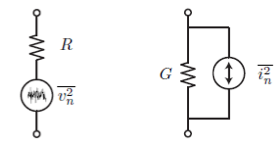
\includegraphics[width=4cm, valign=t]{pictures/widerstandrauschen.png}
    & {	\vspace{-1.8\topsep}
        \begin{align*}
            S_{noise}(R) &=4kTR \qquad [\mathrm{V^2/Hz}]\\
            E_{noise}(R) &=\sqrt{4kTR} \qquad [\mathrm{V/\sqrt{Hz}}]\\
            \overline{v^2_{n}} &=4kTRB = \int_0^{ENB} 4kTR \; df\\
            \overline{i^2_{n}} &=4kTGB = \int_0^{ENB} 4kTG \; df\\
            v_{rms} &= \sqrt{\overline{v^2_{n}}} = \sqrt{4kTRB}
        \end{align*}
      }
    & {B: Bandbreite\newline
       T:  Temperatur in Kelvin (typ: 293K $\hat{=}20^{\circ}$C)\newline
       k:  $1.38 \cdot 10^{-23}JK^{-1}$\newline
       $S_{noise}(R)$:  Spektrale Dichte (Leistungsdichte)\newline
       $E_{noise}(R)$: Rauschspannungsdichte\newline
       $v_{RMS}$:  Rauschspannung\newline
       $ENB$: Effective Noise Bandwidth
      }
    \\ \hline
% ----------------------------------------------------------------------------------------------------   
    \multicolumn{3}{|l|}{\textit{Widerstände in Serie}}
    \\ \hdashline
    \begin{circuitikz}[european, scale=2]
	\draw (0,0) to [R=$R1$, *-] (1,0) to [R=$R2$, -*] (2,0);
\end{circuitikz}
    & {	\vspace{-1.6\topsep}
        \begin{align*}
            \overline{v^2_{n}}&=4kT(R1+R2)B=\overline{v^2_{n1}}+\overline{v^2_{n2}}\\
            \overline{i^2_{n}}&=4kT(G1+G2)B=\overline{i^2_{n1}}+\overline{i^2_{n2}}
        \end{align*}
    }
    & 
    \\ \hline
\end{longtable}
% ----------------------------------------------------------------------------------------------------  
\vspace*{-0.5cm}\begin{longtable}[t]{|p{4cm}|p{5.2cm}|p{7cm}|}    
    \hline 
    \multicolumn{3}{|l|}{\textit{Spannungsteiler}}
    \\ \hdashline
    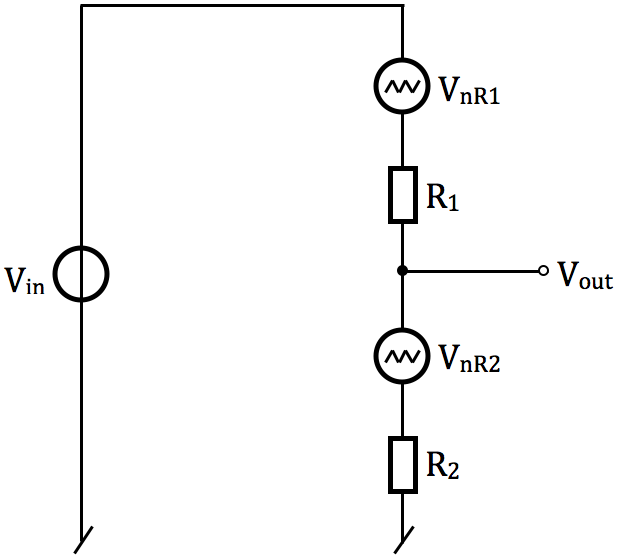
\includegraphics[width=4cm, valign=t]{pictures/RauschenSpannungsteiler.png}
    & {\begin{align*}
            \intertext{Superposition der einzelnen Spannungsquellen}
            V_{out}(V_{in}) &= V_{in} \cdot \frac{R_2}{R_1 + R_2}\\
            V_{out}(V_{nR1}) &= V_{nR1} \cdot \frac{R_2}{R_1 + R_2}\\
            V_{out}(V_{nR2}) &= V_{nR2} \cdot \frac{R_1}{R_1 + R_2}
        \end{align*}
      }
    & {\begin{align*}
            V_{n_{out}}^2 &= \left[ S_{R_1}\left( \frac{R_2}{R_1 + R_2}\right) ^2 + S_{R_2}\left( \frac{R_1}{R_1 + R_2}\right) ^2\right] B \\
            &= 4kT\left( R_1 \frac{R_2^2}{(R_1+R_2)^2} + R_2 \frac{R_1^2}{(R_1+R_2)^2}\right) B\\
            &= 4kT \cdot \frac{R_1 \cdot R_2}{R_1 + R_2}\cdot B\\
            V_{n_{out}} &= \sqrt{\mathrel{\mathop{V_{nR1}^2}\limits_{\substack{\uparrow\\\hbox to 0pt{\hss{\textcolor{red}{\tiny $4kT R_1 B$}}\hss}}}} \left( \frac{R_2}{R_1+R_2}\right) ^2 + \mathrel{\mathop{V_{nR2}^2}\limits_{\substack{\uparrow\\\hbox to 0pt{\hss{\textcolor{red}{\tiny $4kT R_2 B$}}\hss}}}} \left( \frac{R_1}{R_1+R_2}\right) ^2}\\
            &= \sqrt{4kT \cdot \frac{R_1 \cdot R_2}{R_1 + R_2}\cdot B}
        \end{align*}
      }
    \\ \hdashline
    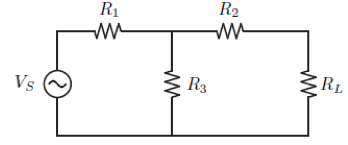
\includegraphics[width=2.8cm, valign=t]{pictures/seriewiderstand1.png}\newline
    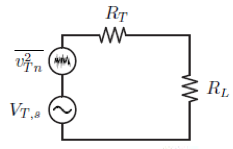
\includegraphics[width=2.5cm]{pictures/seriewiderstand2.png}
    & {Quellenumwandlung machen und dann Rauschen über Ersatzwiderstand ($R_T$) bestimmen.\newline
      }
    & {
	    \begin{align*}
           V_{T,s}&=V_{s}\frac{R_{3}}{R_{1}+R_{3}}\\
           \overline{v^2_{Tn}}&=4kTR_{T}B\\
           &=4kT(R_{2}+R_{1}\parallel R_{3})B
        \end{align*}
      }
    \\ \hline
% ----------------------------------------------------------------------------------------------------       
    \multicolumn{3}{|l|}{\textit{Rauschen von RC-Netzwerken}}
    \\ \hdashline
    \begin{center} \begin{circuitikz}[european]
	\ctikzset{bipoles/length=1cm}
	\draw (0,0) node[ocirc] {} 
		to[short] ++(1,0) node[circ] {}
		to[short] ++(1.3,0)
		to[C=C] ++(0,-1.5)
		to[short] ++(-1.3,0) node[circ] {}
		to[short] ++(-1,0) node[ocirc] {};
	\draw (1,0) to[R=G] (1,-1.5);
	\draw[->] (-0.2,-1.9) node[below] {$\underline{Z}$} -- ++(0,1.2) -- ++(0.4,0);
\end{circuitikz} \end{center}
    & { \vspace{-1.5\topsep}
        \begin{align*}
            H(j\omega) &= \underline{Z}=\frac{1}{G+j\omega C}=\frac{G-j\omega C}{G^2+\omega^2C^2}\\
            \overline{v_{n}} &=\sqrt{\overline{v^2_{n}}} = \sqrt{\overline{i_n^2} \cdot |\underline{Z}|^2}\\ &=\sqrt{\frac{4kTG}{2\pi}\int^{\infty}_{0}\frac{1}{G^2+\omega^2C^2}d\omega}\\
            &=\sqrt{\frac{kT}{C}}            
        \end{align*}
      }
    & {\vspace{-1.5\topsep}
        \begin{itemize}[leftmargin=*]
            \item Kapazitäten (und Induktivitäten) rauschen nicht!
            \item Kapazitäten (und Induktivitäten) ändern die Bandbreite des Systems, d.h. beeinflussen dadurch die Rauschspannung
            \item Der Widerstand trägt nicht direkt zur Rauschspannung bei, er limitiert die Bandbreite
            \newline
        \end{itemize}
      }
    \\ \hline
\end{longtable}
% ----------------------------------------------------------------------------------------------------    
\vspace{-2.5\topsep}
\begin{longtable}[t]{|p{4cm}|p{5.5cm}|p{7.8cm}|}
    \hline  
    \multicolumn{3}{|l|}\textbf{ Berechnung der Rausch-Spannung}
    \\ \hdashline
    Die Rausch-Spannung ist das Integral der Rauschspannungsdichte über den ganzen Frequenzbereich
    & {\vspace{-1.5\topsep}
       \begin{align*}
            \intertext{für weisses Rauschen}
            \overline{V_n^2} &= \int_{f_L}^{f_H} C \, df = \underbrace{C}_{4kT\cdot R} (f_H-f_L) \\
            \intertext{für 1/f-Rauschen}
            \overline{V_n^2} &= \int_{f_L}^{f_H} \frac{K^2}{f} \, df = K^2 \ln\frac{f_H}{f_L}
       \end{align*}
      }
    & {C: Rauschleistungsdichte pro Hertz (konstant)\newline
       \newline\newline\newline
       K: Bauteil-Konstante (in Volt)
      }
    \\ \hline
\end{longtable}

% ----------------------------------------------------------------------------------------------------    
\vspace{-2.5\topsep}
\begin{longtable}[t]{|p{4cm}|p{8cm}|p{5.3cm}|}
    \hline  
    \multicolumn{3}{|l|}\textbf{ Berechnung der Rausch-Spannung (am Beispiel von Tiefpass 1. Ordnung)}
    \\ \hdashline
    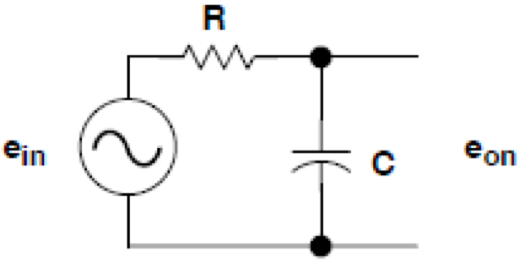
\includegraphics[width=4cm, valign=t]{pictures/RauschenTiefpass.png}
    & {\vspace{-1.5\topsep}
        \begin{align*}
            e_{on} &= \sqrt{\int_{0}^{\infty} \left| A_{n(f)}\right| ^2 e_{in}^2 \, df}\\
            A_{n(f)} &= \frac{1}{1+ j2\pi fRC} \Rightarrow \left| A_{n(f)}\right| ^2 = \frac{1}{1+(2\pi fRC)^2}\\
            e_{on} &= e_{in} \sqrt{\int_{0}^{\infty} \frac{1}{1 + (2\pi fRC)^2}df} = e_{in} \sqrt{\underbrace{\frac{1}{2\pi RC}\frac{\pi}{2}}_{\textcolor{red}{ENB}}}\\
            &= e_{in} \sqrt{\frac{1}{4RC}}
        \end{align*}
        \begin{tabbing}
            \textbf{ Filter-Ordnung}\qquad \= \textbf{ \textcolor{red}{ENB}}\\
            1 \> $1.57 \cdot f_c$\\
            2 \> $1.11 \cdot f_c$\\
            3 \> $1.05 \cdot f_c$\\
            4 \> $1.025 \cdot f_c$
        \end{tabbing}
      }
    & {\textbf{ $e_{on}$}: Rauschspannung am Ausgang der Schaltung\newline\newline
       \textbf{ $e_{in}$}: Rauschspannung am Eingang der Schaltung\newline\newline
       \textbf{ $f_c$}: 3dB-Frequenz \newline\newline
       \textbf{ \textcolor{red}{ENB}}: Effective Noise Bandwidth\newline
       Es wird nicht die 3dB-Bandbreite, sondern das gesamte integrierte Rauschen berechnet
      }
      \\
     \hline
\end{longtable}
% ----------------------------------------------------------------------------------------------------    
\vspace{-2.5\topsep}
\begin{longtable}[t]{|p{4cm}|p{13.8cm}|}
    \hline  
    \multicolumn{2}{|l|}\textbf{ Rauschen in Opamps}
    \\ \hdashline
    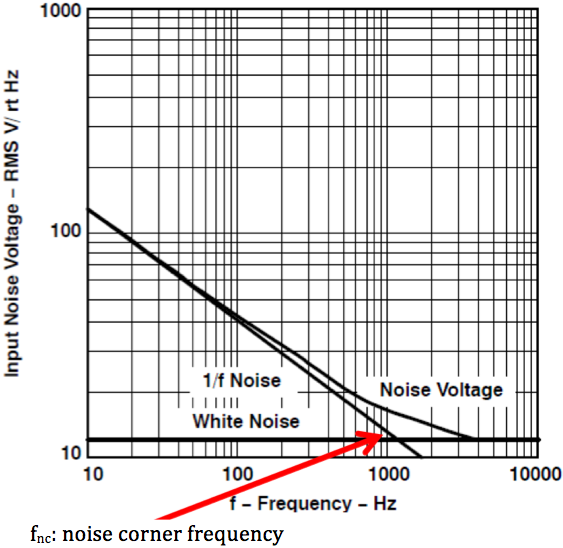
\includegraphics[width=4cm, valign=t]{pictures/NoiseCornerFreq.png}\newline \vspace{0.5cm}\newline
    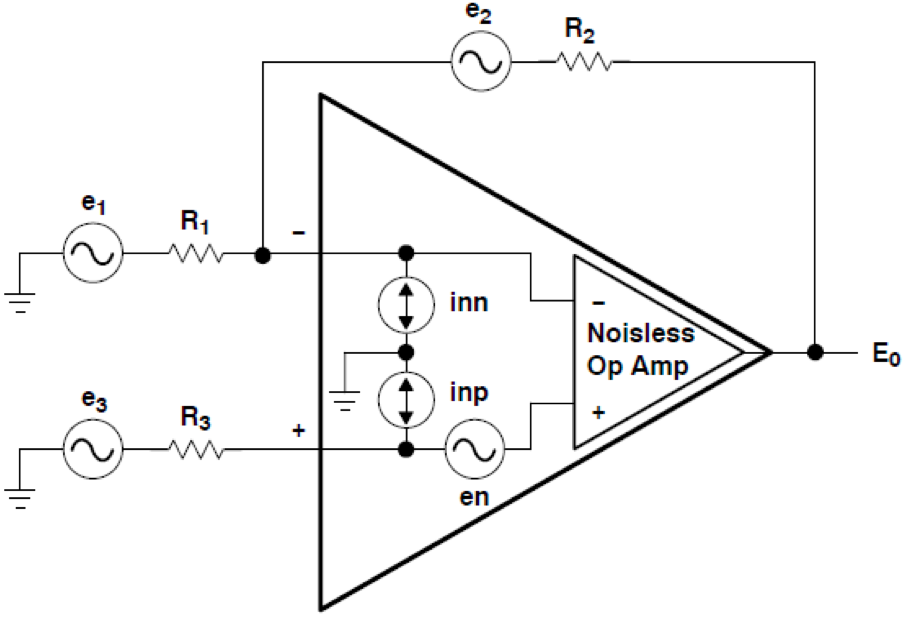
\includegraphics[width=4cm]{pictures/oampnoise.png} \newline \vspace{0.5cm} \newline
    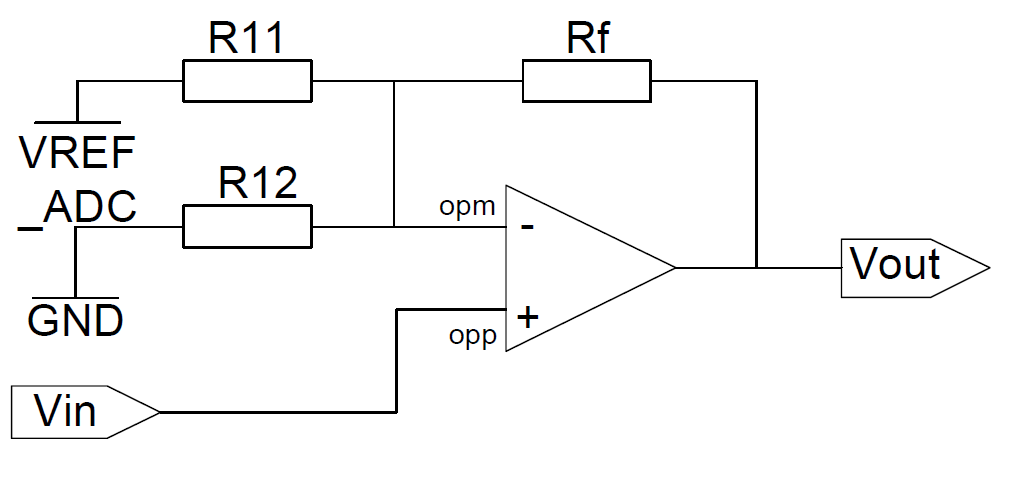
\includegraphics[width=4cm]{pictures/RauschenSummierer}
    &{\textbf{Vorgehen zur Bestimmung der Rauschspannung:}
    \begin{enumerate}
      \setlength{\itemsep}{4pt}
      \item  Verstärkungen bestimmen: \newline
             $\boxed{V_{out} = A_{OP} \cdot V_{in} + A_{ref} \cdot V_{ref} + A_{gnd} \cdot V_{gnd}}$
      \item  \textbf{GBW} bestimmen
      \item  Effektive Rausch-Bandbreite bestimmen: \newline $\boxed{ENB = \dfrac{GBW}{A_{OP}} \cdot \dfrac{\pi}{2}} $
      \item  Eingangsrauschspannungsdichte bestimmen
      \item  auf den Ausgang projizieren: $\boxed{E_{out} = E_{in} \cdot A}$ 
      \item  $\boxed{E_{out_{tot}} = \sqrt{E_1^2 + E_2^2 + \ldots}}$
      \item  Ausgangsrauschspannung: $\boxed{V_{n_{out}} = E_{out_{tot}} \cdot \sqrt{ENB}}$
    \end{enumerate}

    Grundsätzlich gilt, jede Rauschspannungsquelle einzeln betrachten und auf den Ausgang projizieren. 
    \newline
    \newline
    $E$: Rauschspannungsdichte $[V/\sqrt{Hz}]$ \newline
    $V_n$: Rauschspannung $[V]$ \newline
    
    \textbf{Beispiel zum untersten Bild:} \newline
    $V_{out} = \underbrace{\frac{R_f + R_1}{R_1}}_{A_{OP}} \cdot V_{in} - \underbrace{\frac{R_f}{R_{11}}}_{A_{ref}}
    \cdot V_{ref} - \underbrace{\frac{R_f}{R_{12}}}_{A_{gnd}} \cdot V_{gnd}$ \qquad mit $R_1 = R_{11} || R_{12}$ \newline
    $E_{R_{11}out} = A_{ref} \cdot \sqrt{4k \cdot T \cdot R_{11}} \qquad  \qquad E_{R_fout} = \sqrt{4k \cdot T \cdot R_f}$
    }
    \\ \hline
\end{longtable}    
    
\newpage


% ----------------------------------------------------------------------------------------------------    
\vspace{-2.5\topsep}
\begin{longtable}[t]{|p{9cm}|p{9cm}|}
  \hline  
    \multicolumn{2}{|l|}\textbf{ Signal-Rauschabstand (SNR)} \\
  \hdashline
    \vspace{-1.5\topsep}
    \[ P_{sig} = \left(\frac{A_{max}}{c}\right)^2=\left(\frac{2^{n-1}\cdot q}{\sqrt 2}\right)^2 = 2^{2n-3}\cdot q^2\]    
    \newline
    \[ P_Q \approx \frac{q^2}{12} \] \newline
    \[ q = \frac{V_{Refp}-V_{Refn}}{2^n} \]  \newline
    \[ SNR_{db} = 10 \cdot \log\left(\frac{P_{sig}}{P_Q}\right) = 1.76+n \cdot 6.02 \] &
    \vspace{-1.5\topsep}
    \begin{itemize}
      \item[c:] Crestfaktor (Sinussignal $c=\sqrt 2$)
      \item[q:] Quantisierungsintervall
      \item[$P_{sig}$:] Signalleistung
      \item[$P_Q$:] Quantisierungsrauschleistung
      \item[SNR:] Signal to Noise Abstand
    \end{itemize} \\
  \hline
\end{longtable}
    
    
    